\begin{figure}[ht]
  \centering
\begin{adjustbox}{max size={.49\textwidth}}
    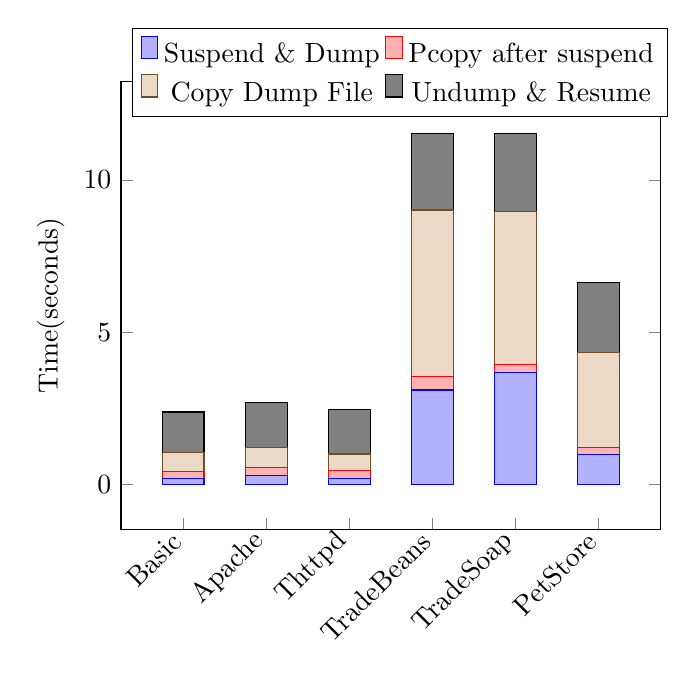
\begin{tikzpicture}
      \begin{axis}[
        ybar stacked,
        bar width=15pt,
        %	nodes near coords,
        enlargelimits=0.15,
        legend style={at={(0.02,1.12)},anchor=north west,legend columns=2},
        ylabel={Time(seconds)},
        symbolic x coords={Basic, Apache, Thttpd, TradeBeans, TradeSoap, 
          PetStore},
        xtick=data,
        x tick label style={rotate=45,anchor=east},
        ]
        \addplot+[ybar] plot coordinates {(Basic,0.21) (Apache,0.30) (Thttpd,0.21) (TradeBeans,3.10) (TradeSoap,3.68) (PetStore,0.97) };
        \addplot+[ybar] plot coordinates {(Basic,0.22) (Apache,0.27) (Thttpd,0.26) (TradeBeans,0.44) (TradeSoap,0.25) (PetStore,0.24) };
        \addplot+[ybar] plot coordinates {(Basic,0.62) (Apache,0.64) (Thttpd,0.53) (TradeBeans,5.47) (TradeSoap,5.03) (PetStore,3.11) };
        \addplot+[ybar] plot coordinates {(Basic,1.33) (Apache,1.47) (Thttpd,1.46) (TradeBeans,2.51) (TradeSoap,2.57) (PetStore,2.32) };
        \addlegendentry{\strut Suspend \& Dump}
        \addlegendentry{\strut Pcopy after suspend}
        \addlegendentry{\strut Copy Dump File}
        \addlegendentry{\strut Undump \& Resume}
        %	\legend{\strut Suspend + Dump, \strut Pcopy after suspend, \strut Copy Dump File, \strut Undump and Resume}
      \end{axis}
    \end{tikzpicture}
  \end{adjustbox}
  \captionsetup{justification=centering}
  \caption{Suspend time for live cloning, when running a representative benchmark}
  \label{fig:stats}
\end{figure}



%\begin{figure*}[ht]
%\centering
%\begin{minipage}[b]{0.45\textwidth}
%\end{minipage}
%\quad
%\begin{minipage}[b]{0.45\textwidth}
%\end{minipage}
%\end{figure*}

\noindent
\textbf{Real-World application, and workloads:}
%To evaluate the suspend time in real-world scenarios, we tested our cloning operation on real-world applications, running a realistic workload.
In figure~\ref{fig:stats}, we show the suspend times for five well known applications - Apache, Thttpd, TradeBeans, TradeSoap, PetStore. 
%both internal and external mode while comparing it with a production container, that is idle vs. a container which is running an apache hog benchmark \cite{httperf} on it. 
For Apache, and thttpd which are web-servers, we ran the httperf~\cite{httperf} hog benchmark. 
The hog benchmark tries to compute max throughput of the web-server, by sending a large number of concurrent requests.
Tradebeans and Tradesoap are both part of the dacapo~\cite{dacapo} benchmark ``DayTrader'' application.
These are realistic workloads, which run on a multi-tier trading application provided by IBM. 
PetStore~\cite{petstore} is a well known J2EE reference application. 
We deployed PetStore in a 3-tier system with JBoss, MySQL and Apache servers.
Here we cloned the app-server, and the input workload was a random set of transactions which were repeated for the duration of the cloning process.
%For MySQL we ran a similar workload with some read and write queries to test how well our cloning operation performs.
We found that for hog benchmarks, the container suspend time was 2-3 seconds.
However, for heavy workloads in more memory intensive application servers such as PetStore, DayTrader, the total suspend time was higher (6-12 seconds).
We found that we did not experience any timeouts or errors for the requests in the workload\footnote{In case of packet drops, requests are resent both at the TCP layer, and the application layer. This slows down the requests for the user, but does not drop them}.
However, this did slowdown requests in the workload. 
This confirmed our hypothesis that short suspend times are largely not visible/have minimal performance impact to the user, as they are within the time out range of most applications.
Further a clean network migration process ensures that connections are not dropped, and the workload is executed successfully.
